\section{The \shortname protocol}\label{sect:model}


\begin{figure}[tp]
	\centering
	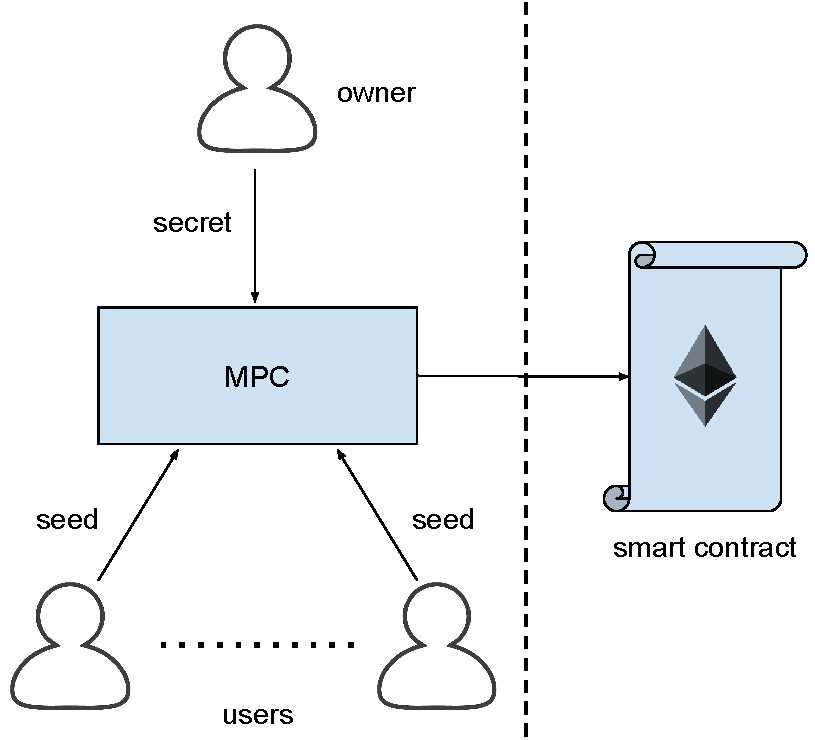
\includegraphics[width=0.6\textwidth]{fig/proposal}
	\caption{\name (\shortname) reference diagram.}
	\label{fig:model}
\end{figure}

%\subsection{Terminology}

%We describe \shortname's  protocol using the following terminology:

%\para{Secret}
%A secret \secret represents the information to be protected.

%\para{Time-Lock ({\em TL})}
%
%A \textit{Time-Lock} is a mechanism that keeps the secret \secret private until its {\em disclosure time} \td.
%
%The \textit{Time-Lock} publishes \secret{}  after \td.

%\para{Owner}
%An owner \owner is someone who wraps a secret \secret using a Time-Lock.
%
%The owner delegates the disclosure of \secret to the Time-Lock, i.e., the owner is \textit{not} involved in the disclosure of \secret at \td.


% By creating the Time-Lock, the owner delegates the disclosure of the secret to the TL, thus effectively decoupling himself from the disclosure process (i.e., the secret will be revealed at \td without requiring the owner to play an active role in the process after the setup).

%\begin{description}
%
%	\smallskip
%    \item [Secret] --- A secret \secret represents the information to be protected.
%
%	\smallskip
%    \item [Time-Lock ({\em TL})] --- A Time-Lock is a mechanism used to keep the secret \secret private until its {\em disclosure time} \td and then publish it unconditionally.
%
%	\smallskip
%    \item [Owner] --- The owner \owner is someone who wants to wrap a secret \secret using the Time-Lock. By creating the Time-Lock, the owner delegates the disclosure of the secret to the TL, thus effectively decoupling himself from the disclosure process (i.e., the secret will be revealed at \td without requiring the owner to play an active role in the process after the setup).
%
%\end{description}
%\smallskip

%\shortname implements a Time-Lock by distributing the secret \secret among several users so that no single user has access to \secret before the disclosure time \td.

%Concretely, the secret \secret is split into \N shares \share using Shamir's secret sharing~\cite{Shamir:1979:SS:359168.359176}.
%%
%Each share is entrusted to a \textit{shareholder} \shareholder.
%
%
%in such a way that it is possible to reconstruct \secret by combining \K different shares (i.,e., using Shamir's method~\cite{Shamir:1979:SS:359168.359176}).


%\begin{description}

	%\smallskip
    %\item [Share] --- The secret \secret is divided into \N shares ${\share}_1,\dots,{\share}_n$ in such a way that it is possible to reconstruct \secret by combining \K different shares (i.,e., using Shamir's method~\cite{Shamir:1979:SS:359168.359176}).

	%\smallskip
    %\item [Shareholder] --- A shareholder \shareholder is the subject entrusted to store a share in such a way that no other party can access it before the disclosure time. After \td, the shareholders publish their shares so that anyone can reconstruct the secret \secret.

%\end{description}

ITYT is an instance of the TL abstraction: a mechanism that keeps a secret \secret private until its {\em disclosure time} \td and publishes it afterwards.
%
\shortname implements TL by distributing the secret, provided by the {\em owner}, among several users (named {\em shareholders}, each obtaining a share \share), so that a single user can't see  \secret before the disclosure time \td.

\shortname leverages economic incentives and penalties to ensure that (i) each user keeps its share secret until \td, and (ii) users disclose the shares to reconstruct the secret after \td.
%
%As we show in Section~\ref{??}, if the users behave as rational economic agents, then \shortname effectively implements the TL abstraction.
%
%Rather than relying on trusted third parties~\cite{?} or Proof-of-Work~\cite{?}, \shortname implements a TL in a distributed fashion by relying on economic incentives.
%
\shortname achieves practical Time-Locks as a consequence of the rational economic behavior of the involved parties
(see Section~\ref{sect:constraints}).
%In the remainder of this section we present the \shortname protocol as regards the roles, the parameters, and the protocols.

\subsection{Definitions}

\subsubsection*{Principals}
We denote by \users the set of users that take part in an instance of \shortname.
Additionally we denote by \smartcontracts the set of the smart contract identifiers.
We then denote by \principals the set of principals consisting of $\users \cup \smartcontracts$.

\medskip

\subsubsection*{Wallets}
Each principal $p \in \principals$ is associated with a wallet $\wallet{p}$, accessible only by $p$, that can be used to receive or issue payments.

\medskip

\subsubsection*{Protocol parameters}
This table references to all the parameters that characterize an instance of the \shortname protocol. \\

\begin{tabular}{ll}
	\secret & secret \\
	\V & value of the secret \\
	$\share_{i}$ & share of the secret issued to the $i$-th shareholder \\
	\N & number of shareholders \\
	\K & number of shares needed to reconstruct \secret \\	
	\td & disclosure time \\
	\te & termination time \\
	\PO & pawn deposited by the owner \\
	\BH & bid deposited by the shareholder \\
	\RH & reward paid to the shareholder in case of success \\
	\Wshare & reward paid when whistleblowing a share \\
	\Wsecret & reward paid when whistleblowing the secret \\

	& \\
\end{tabular}

\subsubsection*{Smart Contract Data}
The \shortname smart contract is a data structure with functions. 
Its initialization and functions will be described in Section~\ref{sect:sc_init} and \ref{sect:sc_functions} respectively. The data structure is composed by the following entries.
Moreover, we will use the notation $sc.x$ to reference to the smart contract variable $x$.

\begin{tabular}{ll}
	& \\
	
	\PO, \BH & economic pawn and bids \\
	\td, \te, \N, \K & technical parameters \\
	\RH, \Wsecret, \Wshare & economic rewards \\
	$\left[ \shares \right]$ & array of deposited shares \\
	\Csecret & commitment of the secret \\
	$\left[ \Cshare \right]$ & array of share commitments \\	
	\state & state of the \shortname protocol \\
	$\left[ \states \right]$& array of states for each share \\
	\numpending & number of pending shareholders \\
	\numdisclosed & number of disclosed shares \\
	& \\
\end{tabular}

\subsubsection*{Primitives}
We now define the primitives used in the \shortname smart contract algorithms.

\begin{asparaitem}
	\item \primtime: 
	returns the current time as witnessed by the blockchain (generally defined in terms of block height).
		
	\item \primhash{d}: 
	returns the result of the application of a chosen cryptographic hash function over the data $d$.
	
	\item \primpay{p_1}{p_2}{v}: 
	transfers $v$ from $\wallet{p_1}$ to $\wallet{p_2}$.
	
	\item \primwithdraw{sc}{p}{v}{predicate}:
	allows principal $p$ to withdraw the amount $v$ from $\wallet{sc}$, if $predicate$ holds. The predicate can also involve time constraints.
	
	\item \primgenerateshares{\secret}{[users]}: 
	generates the shares $\share_1, \ldots, \share_n$ using \KofN secret sharing~\cite{Shamir:1979:SS:359168.359176}, then it securely distributes them to the parties.
	The primitive guarantees that the (a) $i$-th shareholder is the only principal who learns the share $\share_i$, and (b) the owner learns only the commitment $hash(\share_i)$, for all the shares. 
	We discuss in Section~\ref{sect:realization} how our prototype implements this primitive by leveraging sMPC.	
	
	\item \priminit{[params]}: 
	instantiates an \shortname smart contract, with parameters $[params]$, and deploys it to the blockchain.
	The primitive is executed by the owner and returns the smart contract identifier $sc \in \smartcontracts$.

\end{asparaitem}


\begin{algorithm}[t]
	\caption{Protocol initialization (executed by the owner)}\label{algo:init}
	\begin{algorithmic}[1]
		\MyAlgBlock{input}
		\Desc{$[params]$}{\hspace*{4em}economic values of the \shortname instance}
		\Desc{\secret}{\hspace*{4em}secret}
		\Desc{\owner}{\hspace*{4em}user identifier of the owner}
		\Desc{$[\shareholder_{1}, \ldots, \shareholder_{\N}]$}{\hspace*{4em}list of shareholder identifiers}
		\vspace{0.6em}
		
		\Procedure{\algoinit}{$[params],\secret,\owner,[\shareholder_{1}, \ldots, \shareholder_{\N}]$}
		\State $sc\gets \priminit{[params]}$\Comment{Create $sc$}
		\State $\primpay{\owner}{sc}{sc.\PO}$ \Comment{Transfer owner's pawn to $sc$}
		\State $\Cshare{} \gets \primgenerateshares{\secret}{[\owner, \shareholder_{1}, \ldots, \shareholder_{\N}]}$
		\State $sc.\Csecret\gets \primhash{\secret}$ \Comment{Set secret commitment}
		\State $sc.state\gets \statepending$
		\For {$i\gets 1, \N$} \Comment{Set share commitments}
		\State $sc.\Cshare{}[i]\gets \Cshare{}[i]$
		\State $sc.states[i]\gets \statepending$
		\EndFor
		\State $sc.numpending\gets \N$
		\State $sc.numdisclosed\gets 0$
		\State \textbf{return} $sc$\Comment{The smart contract id}
		\EndProcedure	
	\end{algorithmic}
\end{algorithm}


\subsection{Roles}

%
In \shortname, each user $u \in \users$ plays one of the following roles: {\em owner}, or {\em shareholder}. In addition to her role, a user can also play the role of the {\em whistleblower}, needed to enforce the execution of the economic penalties.

\begin{asparaitem}
\item {\bf Owner:}	An owner \owner is someone willing to delegate the disclosure of a secret \secret to a Time-Lock, so that the owner is \textit{not} involved in the disclosure of \secret at disclosure time \td.
The owner \owner sets up the TL as well as the corresponding parameters.
In particular, \owner sets (i) \N the total number of shares \share of \secret, (ii) \K, the number of shares needed to recover \secret, and (iii) all the bids and the rewards that define the instance.

% MG: Is the owner's pawn $\PO$ part of the parameters? If yes, shouldn't we check whether all the bids and rewards are well-formed?
% DF: As the abstraction is based on economic assumptions, a game with incorrect/inconsistent parameters won't be played by anyone. Indeed, shareholders are able to opt out (updated below).
% EB: I added a sentence below in C.

\item {\bf Shareholder:}
A shareholder \shareholder is entrusted by the owner \owner to keep a share \share of the secret \secret confidential until \td, and to publicly disclose it afterwards.
In exchange for her service, $\shareholder_{i}$ will receive a reward paid by the smart contract whenever the following two conditions hold: (i) her share $\share_{i}$ is disclosed only after \td, and (ii) the secret \secret is not revealed before \td.

\item {\bf Whistleblower:}
A whistleblower \whistleblower reports misbehavior in return for economic incentives.
Whenever \whistleblower possesses either a share \share or the secret \secret before \td, \whistleblower can submit it and receive a reward.
\end{asparaitem}


\begin{algorithm}[t]
	\caption{Shareholder commitment to take part to \shortname}\label{algo:shareholder_commitment}
	\begin{algorithmic}[1]
		\MyAlgBlock{input}
		\Desc{$sc$}{\hspace*{1.5em}smart contract identifier}
		\Desc{$i$}{\hspace*{1.5em}index of the current shareholder}
		\Desc{$\shareholder_i$}{\hspace*{1.5em}user identifier of the $i$-th shareholder}
		\vspace{0.6em}
		\Statex{\hspace*{-1em}$\triangleright$ {\bf precondition}: $\shareholder_i$ checks that $\primhash{\share_i} = sc.\Cshare{}[i]$}
		\vspace*{0.6em}
		\Procedure{\algoparticipate}{$sc,i,\shareholder_i$}
		
		\If{$sc.\states[i] = \statepending$}
		\State $\primpay{\shareholder_i}{sc}{sc.\BH}$
		\State $sc.\states[i]\gets \statepaid$
		\State $sc.\numpending\ -= 1$
		\If{$sc.\numpending = 0$}
		\State $sc.\state\gets \statelocked$
		\EndIf
		\EndIf
		\EndProcedure
	\end{algorithmic}
\end{algorithm}

\subsection{Smart contract setup}\label{sect:sc_init}

We assume that the owner already selected the shareholders that will take part to the TL instance\footnote{\ How to randomly choose competing players in adversarial settings such as blockchains has already been addressed by other publications~\cite{dong2017betrayal,10.1007/978-3-030-01177-2_81}.}.
To start the setup, the owner instantiates a smart contract, $sc$ using \priminit{[params]}, where $[params]$ are the desired economic parameters.
%The smart contract will be used to execute actions in place of a trusted party.
Then, by collaborating with the shareholders, she executes the $\texttt{generate\_shares}$ primitive and updates $sc$ with the commitments of the secret and of the shares.
She also transfers the amount \PO to $sc$, used to pay the rewards.
The steps are illustrated in Algorithm~\ref{algo:init}.

A shareholder \shareholder is incentivized in taking part to the TL by the possibility of earning a reward \RH.
Once each shareholder gets the share, she verifies that the corresponding commitment written into $sc$ matches. 
If so, she agrees to deposit her bid, \BH ($<\RH$). 
This process is shown in Algorithm~\ref{algo:shareholder_commitment}.
%
As soon as all the shareholders have executed this algorithm, the state of the instance is set to \statelocked, and the TL is active. 
If not all the parties commit before a defined deadline, the deposited funds are returned to their proprietaries and the instance setup aborts. This will be discussed more in details in Section~\ref{sect:realization}.

The algorithms do not check for the economic parameters to be well-formed (see Section~\ref{sect:constraints}). 
In fact, as all the parameters are public and immutable, a malformed game will not be played by any participant in the same way a lottery whose top prize worth less than the ticket price will not sell tickets.

%Do we really want this paragraph here: {\em The reader may notice that, in this setting, the secret could be recovered before the activation of the TL, because at that time all the share have already been distributed. We emphasize that the current section proposes a high level representation of the protocol. In Section~\ref{sect:ityt_exec} we show how to securely distribute the shares, without exposing \secret until TL activation, while still ensuring the shareholders they will be able to fulfill the commitments.}

\subsection{Smart contract functions}\label{sect:sc_functions}

Before presenting the functions (actions), it is important to note that the intrinsic transaction ordering of the blockchain guarantees that each function invocation is executed atomically, thus locking mechanisms are not required.

%%% WHISTLEBLOWSHARE FUNCTION %%%

\smallskip
\texttt{\algowhistleblowshare}:
This function enables the whistleblower to report the misbehave of a single shareholder.
\whistleblower sends the share $\share_{i}$ to the contract.
If the commitment matches, the share whistleblow bonus $\Wshare$ ($<$$\BH$), is payed to the whistleblower.
In that event, the shareholder $\shareholder_{i}$, would lose the chance of earning her reward, \RH.
Another consequence, is that if the number of whistleblown shares would equal $k$, then the TL would be marked as failed (i.e., no further actions allowed).
The function is presented is Algorithm~\ref{algo:whistleblow_share}.

\begin{algorithm}[t]
	\caption{SC function to whistleblow a share before \td}\label{algo:whistleblow_share}
	\begin{algorithmic}[1]
		\MyAlgBlock{input}
		\Desc{$sc$}{\hspace*{1.5em}smart contract identifier}
		\Desc{$i$}{\hspace*{1.5em}index of the whistleblown share}
		\Desc{$\share_i$}{\hspace*{1.5em}the $i$-th share to be whistleblown}
		\vspace{0.6em}
		\Procedure{\algowhistleblowshare}{$sc, i, \share_{i}$}
		\If{$sc.\state = \statelocked$ \textbf{and} $\primtime < sc.\td$}
		\If{$sc.\states[i] = \statepaid$ }
		\If{$\primhash{\share_i} = sc.\Cshare{}[i]$}
		\State $sc.\shares \left[ i \right] \gets \share_{i}$
		\State $sc.\states[i]\gets \statewblowed$
		\State $sc.\numdisclosed\ += 1$
		\If{$sc.\numdisclosed = sc.\K$}
		\State $sc.\state\gets \statefailed$
		\EndIf
		\State $\primpay{sc}{caller}{sc.\Wshare}$
		\EndIf
		\EndIf
		\EndIf
		\EndProcedure
	\end{algorithmic}
\end{algorithm}

%%% WHISTLEBLOWSHARE FUNCTION %%%

\smallskip
\texttt{\algowhistleblowsecret}:
It enables the whistleblower \whistleblower, to prove the possession of the secret ahead of the disclosure time \td.
In detail, \whistleblower sends a secret, $\secret'$ to the contract.
If the commitment matches, then the TL is marked as failed and the secret whistleblow bonus \Wsecret ($>\RH$) is payed to the whistleblower.
In that event, all the shareholders would be subject to an economic penalty that results in the loss of the bid already paid, and the remaining smart contract funds are destroyed.
The function is illustrated is Algorithm~\ref{algo:whistleblow_secret}.
The need for both \texttt{\algowhistleblowshare} and \texttt{\algowhistleblowsecret} will be discussed in details in Section~\ref{sect:analysis}.

\begin{algorithm}[t]
	\caption{SC function to whistleblow the secret before \td}\label{algo:whistleblow_secret}
	\begin{algorithmic}[1]
		\MyAlgBlock{input}
		\Desc{$sc$}{\hspace*{1.5em}smart contract identifier}
		\Desc{\secret}{\hspace*{1.5em}the secret to be whistleblown}
		\vspace{0.6em}
		\Procedure{\algowhistleblowsecret}{$sc, \secret$}
		\If{$sc.\state = \statelocked$ \textbf{and} $\primtime < sc.\td$}
		\If{$\primhash{\secret} = sc.\Csecret$}
		\State $sc.\state\gets \statefailed$
		\State $\primpay{sc}{caller}{sc.\Wsecret}$
		\EndIf
		\EndIf
		\EndProcedure
	\end{algorithmic}
\end{algorithm}

%%% DISCLOSE FUNCTION %%%

\smallskip
\texttt{\algodisclose}:
After the disclosure time \td has passed, each shareholder $\shareholder_{i}$ submits her share $\share_{i}$ to the contract.
The submission is successful if (a) the TL is not marked as \statefailed, (b) the share is marked as \statepaid, and (c) $\primhash{\share_i}$ matches the value stored into the $sc$, otherwise it fails.
Conditionally to the outcome of the TL instance, and immediately after the termination time \te, the rewards are paid for each shareholder that correctly completed the disclosure procedure.
The disclosure procedure is detailed in Algorithm~\ref{algo:disclose}.